\subsection{三垂线定理}\label{subsec:1-11}

\begin{dingli}[三垂线定理][dl:scx]
    在平面内的一条直线,如果和这个平面的一条斜线的射影垂直,那么它也和这条斜线垂直。
\end{dingli}

\begin{wrapfigure}[5]{r}{5cm}
    \centering
    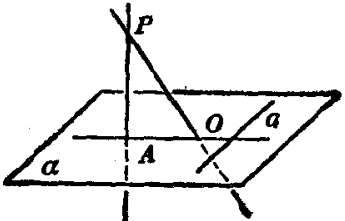
\includegraphics[width=5cm]{../pic/ltjh-ch1-34.png}
    \caption{}\label{fig:ltjh-1-34}
\end{wrapfigure}

已知:$PA$、$PO$ 分别是平面 $\alpha$ 的垂线、斜线, $AO$ 是 $PO$ 在平面 $\alpha$ 上的射影。
$a \subset \alpha$, $a \perp AO$ (图 \ref{fig:ltjh-1-34})。

求证: $a \perp PO$。

\zhengming

$\left.\begin{aligned}
    \left.\begin{aligned}
        \left.\begin{aligned}
            PA \perp \alpha \\
            a \subset \alpha
        \end{aligned}\right\}  \tuichu  PA \perp a \\
        AO \perp a
    \end{aligned}\right\}  \tuichu  a \perp \text{平面}\; PAO \\
    PO \subset \text{平面}\; PAO
\end{aligned}\right\}  \tuichu  a \perp PO \juhao$
\jiange

三垂线定理实质上是平面的一条斜线和平面内的一条直线垂直的判定定理。
这两条直线可以是相交直线,也可以是异面直线。

类似地可以证明:

\begin{dingli}[三垂线定理的逆定理][dl:scx-ndl]
    在平面内的一条直线,如果和这个平面的一条斜线垂直,那么它也和这条斜线的射影垂直。
\end{dingli}

三垂线定理及其逆定理,可以改写成:平面内的一条直线和这个平面的一条斜线垂直的充要条件是它和斜线在平面上的射影垂直。


\liti 如果一个角所在平面外一点到角的两边距离相等,那么这一点在平面上的射影在这个角的平分线上。

已知: $\angle BAC$ 在平面 $\alpha$ 内,点 $P \not \in \alpha$, $PE \perp AB$,
$PF \perp AC$, $PO \perp \alpha$, 垂足分别是 $E$、$F$、$O$, $PE = PF$(图 \ref{fig:ltjh-1-35})。

求证: $\angle BAO = \angle CAO$。

\zhengming

$\left.\begin{aligned}
    \left.\begin{aligned}
        PE = PF \\
        PO \perp \alpha
    \end{aligned}\right\}  \tuichu OE = OF \\
    \left.\begin{aligned}
        PO \perp \alpha \\
        PE \perp AB \\
        PF \perp AC
    \end{aligned}\right\}  \tuichu  \left\{\begin{aligned}
        OE \perp AB \\
        OF \perp AC
    \end{aligned}\right.
\end{aligned}\right\}  \tuichu  \angle BAO = \angle CAO \juhao$

\begin{figure}[htbp]
    \centering
    \begin{minipage}[b]{7cm}
        \centering
        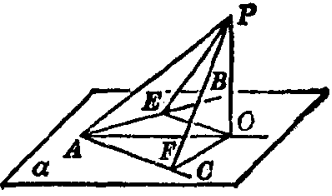
\includegraphics[width=5cm]{../pic/ltjh-ch1-35.png}
        \caption{}\label{fig:ltjh-1-35}
    \end{minipage}
    \qquad
    \begin{minipage}[b]{7cm}
        \centering
        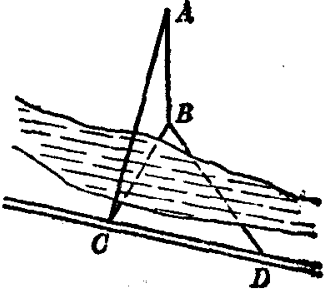
\includegraphics[width=4cm]{../pic/ltjh-ch1-36.png}
        \caption{}\label{fig:ltjh-1-36}
    \end{minipage}
\end{figure}

% \jiange
\liti 道旁有一条河,彼岸有电塔 $AB$,高 15 m。只有测角器和皮尺作测量工具,能否求出电塔顶与道路的距离?

\jie 图 \ref{fig:ltjh-1-36},在道边取一点 $C$, 使 $BC$ 与道边所成的水平角等于 $90^\circ$。
再在道边取一点 $D$,使水平角 $CDB$ 等于 $45^\circ$。
测得 $C$、$D$ 的距离等于 20 m。

$\because$ \quad $BC$ 是 $AC$ 的射影,且 $CD \perp BC$,

$\therefore$ \quad $CD \perp AC$。

因此斜线 $AC$ 的长度就是电塔顶与道路的距离。

$\because$ \quad $\angle CDB = 45^\circ$, $CD \perp BC$, $CD = 20$ m,

$\therefore$ \quad $BC = 20$ m。 由直角三角形 $ABC$:

\qquad $AC^2 = AB^2 + BC^2$, $AC = \sqrt{15^2 + 20^2} = 25$ (m)。

答:电塔顶与道路的距离是25米。


\begin{lianxi}

\xiaoti{已知:点 $O$ 是 $\triangle ABC$ 的垂心, $OP \perp \text{平面}\;ABC$。
    求证: $PA \perp BC$。
}

\xiaoti{在图 \ref{fig:ltjh-1-32} 中,如果 $\theta = 45^\circ$, $\angle BOC = 45^\circ$。
    求 $\angle AOC$,并验证 $\angle AOC > \angle \theta$。
}

\end{lianxi}

